% \documentclass[t]{beamer}
\documentclass{beamer}
\usepackage{minted}
\usepackage{tikz}
\usepackage{amsmath}
\usepackage{adjustbox}

\setminted{fontsize=\footnotesize}


\title{Synchronous single initiator spanning tree algorithm using flooding}
\author{Siddharth Bhat, Anurag Chaturvedi, Hitesh Kaushik}
\date{\today}

\begin{document}
\begin{frame}
\titlepage
\end{frame}

\begin{frame}
    % spanning tree computation: why is it hard in a distributed system
\end{frame}


% algorithm explanation
\begin{frame}
    \frametitle{Example}
    \begin{figure}
    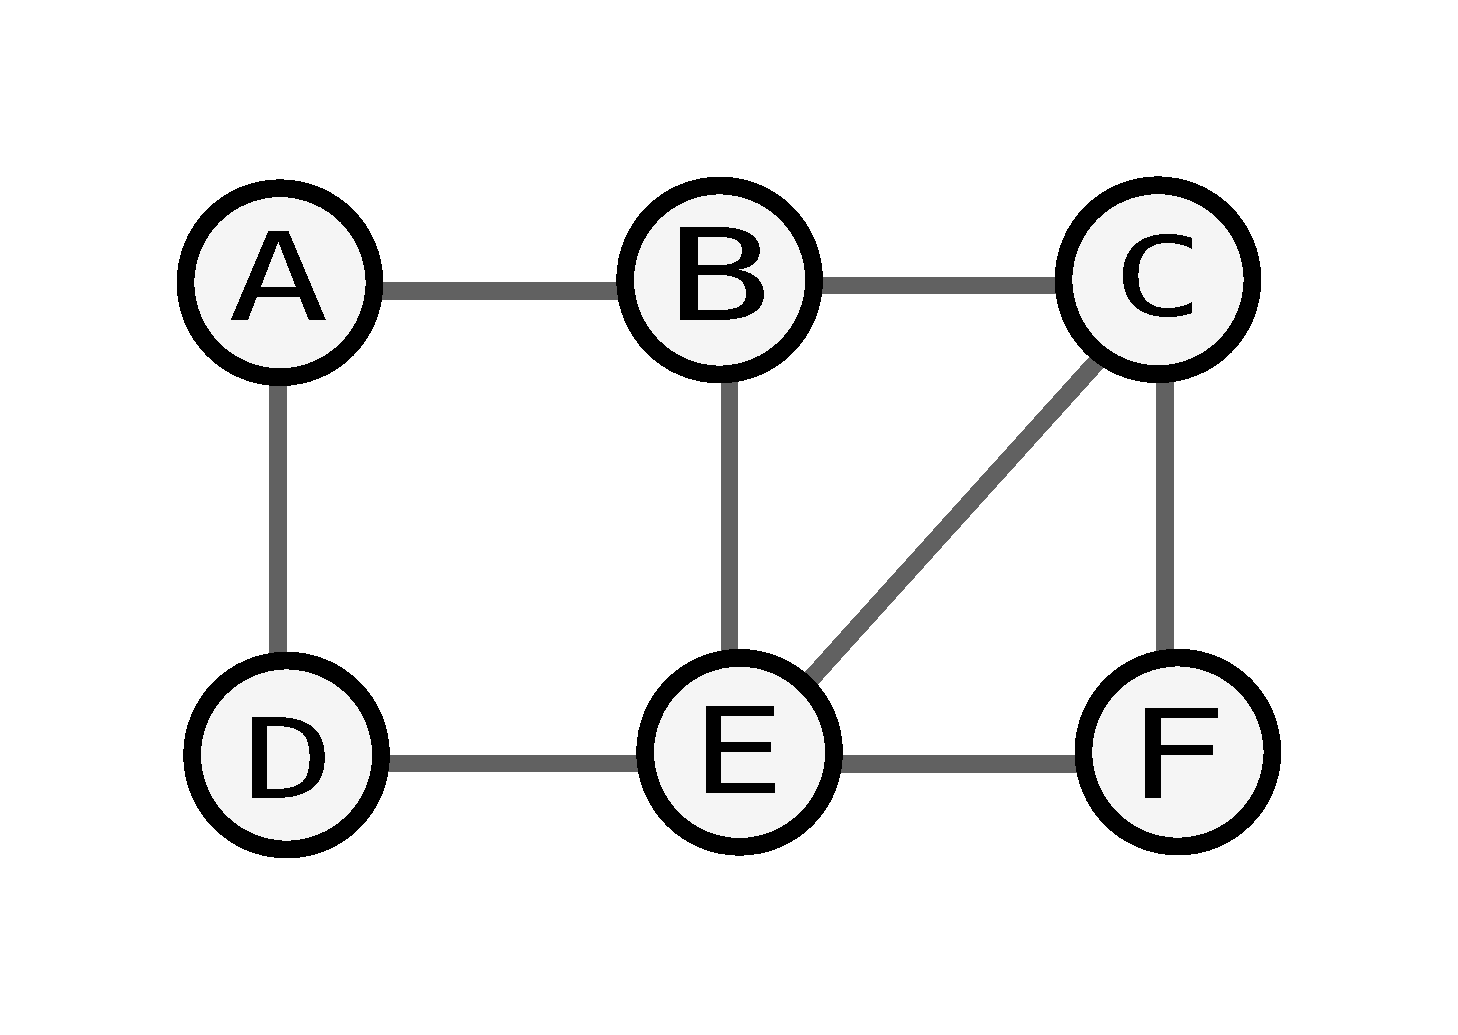
\includegraphics[width=0.5\paperwidth]{base.pdf}
    \end{figure}
\end{frame}

\begin{frame}
    \frametitle{Example}
    \begin{figure}
    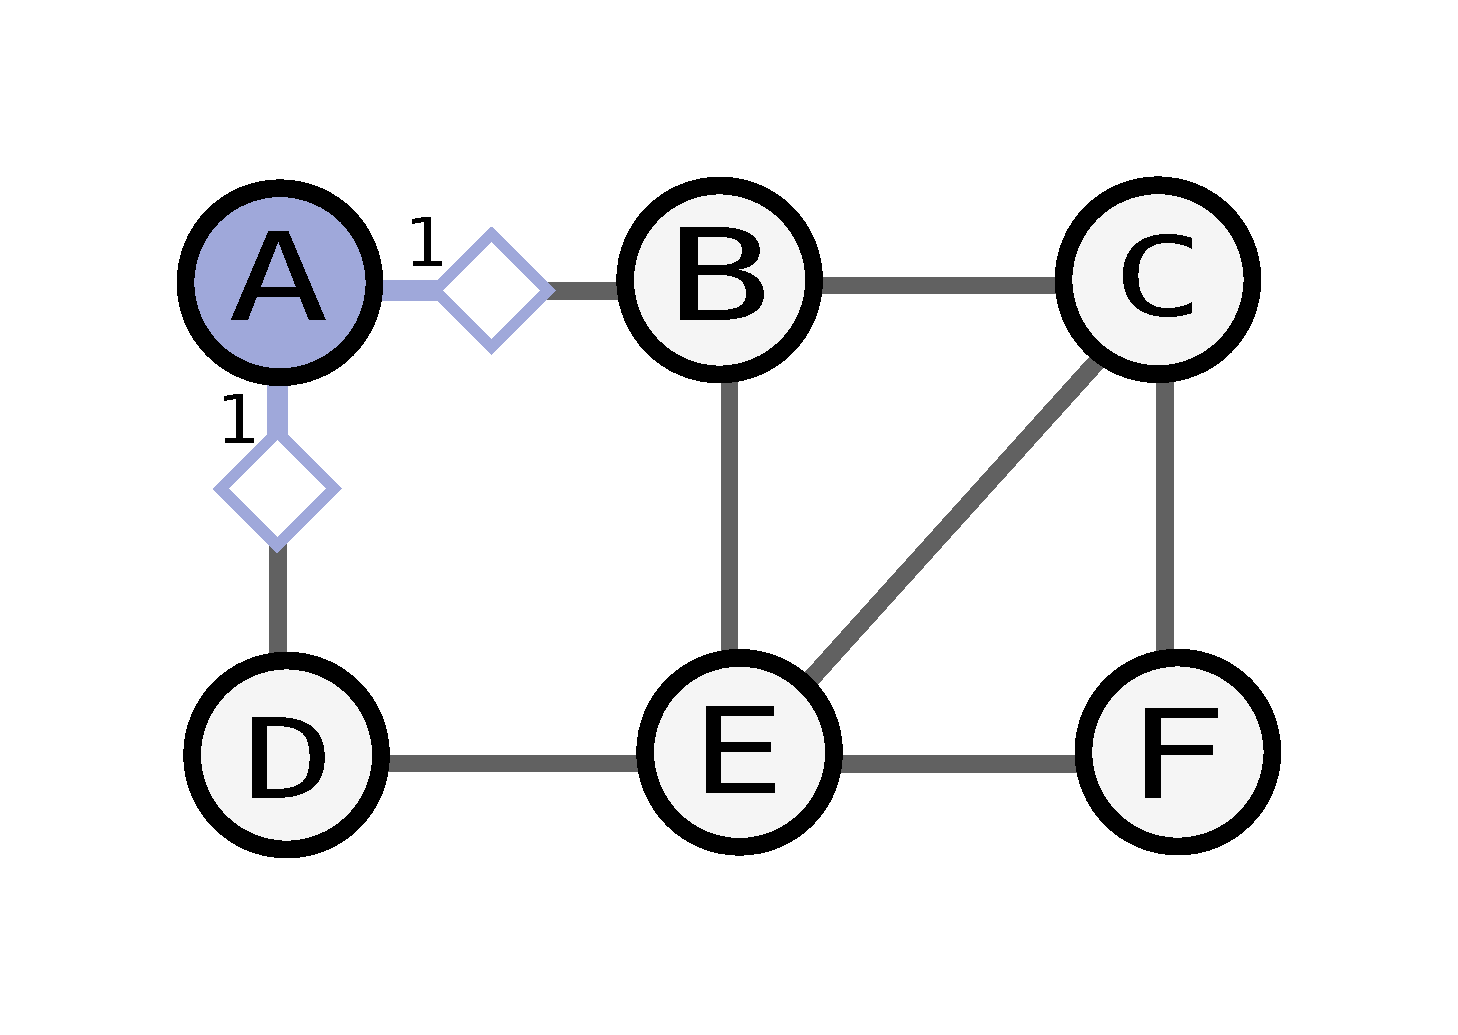
\includegraphics[width=0.5\paperwidth]{round1.pdf}
    \end{figure}
\end{frame}

\begin{frame}
    \frametitle{Example}
    \begin{figure}
    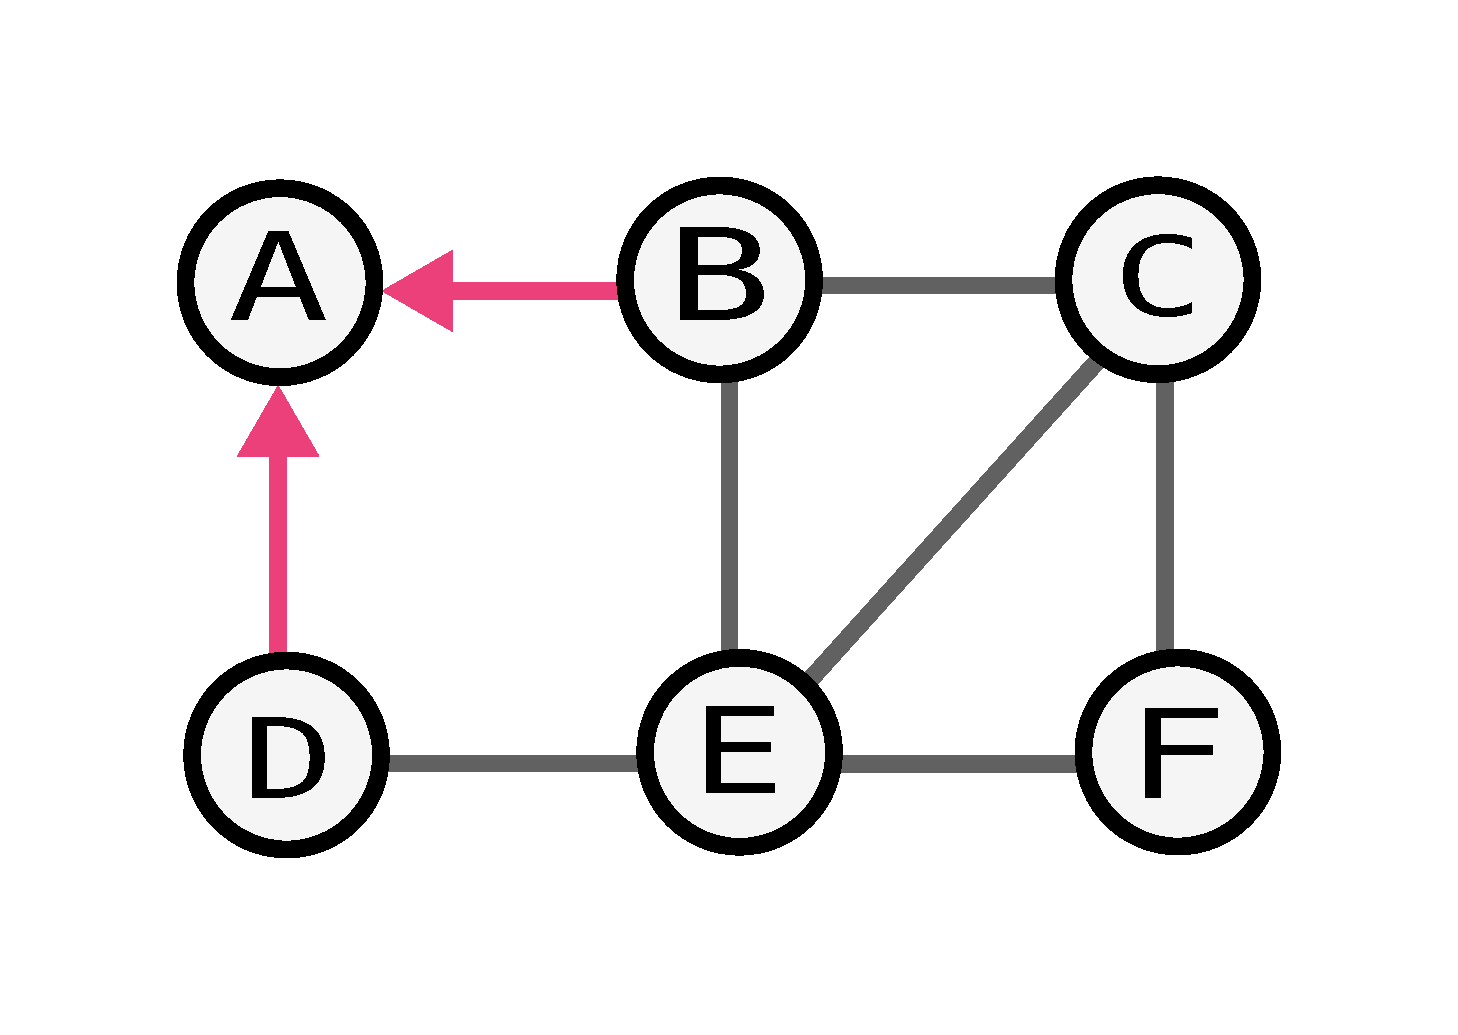
\includegraphics[width=0.5\paperwidth]{round1-end.pdf}
    \end{figure}
\end{frame}


\begin{frame}
    \frametitle{Example}
    \begin{figure}
    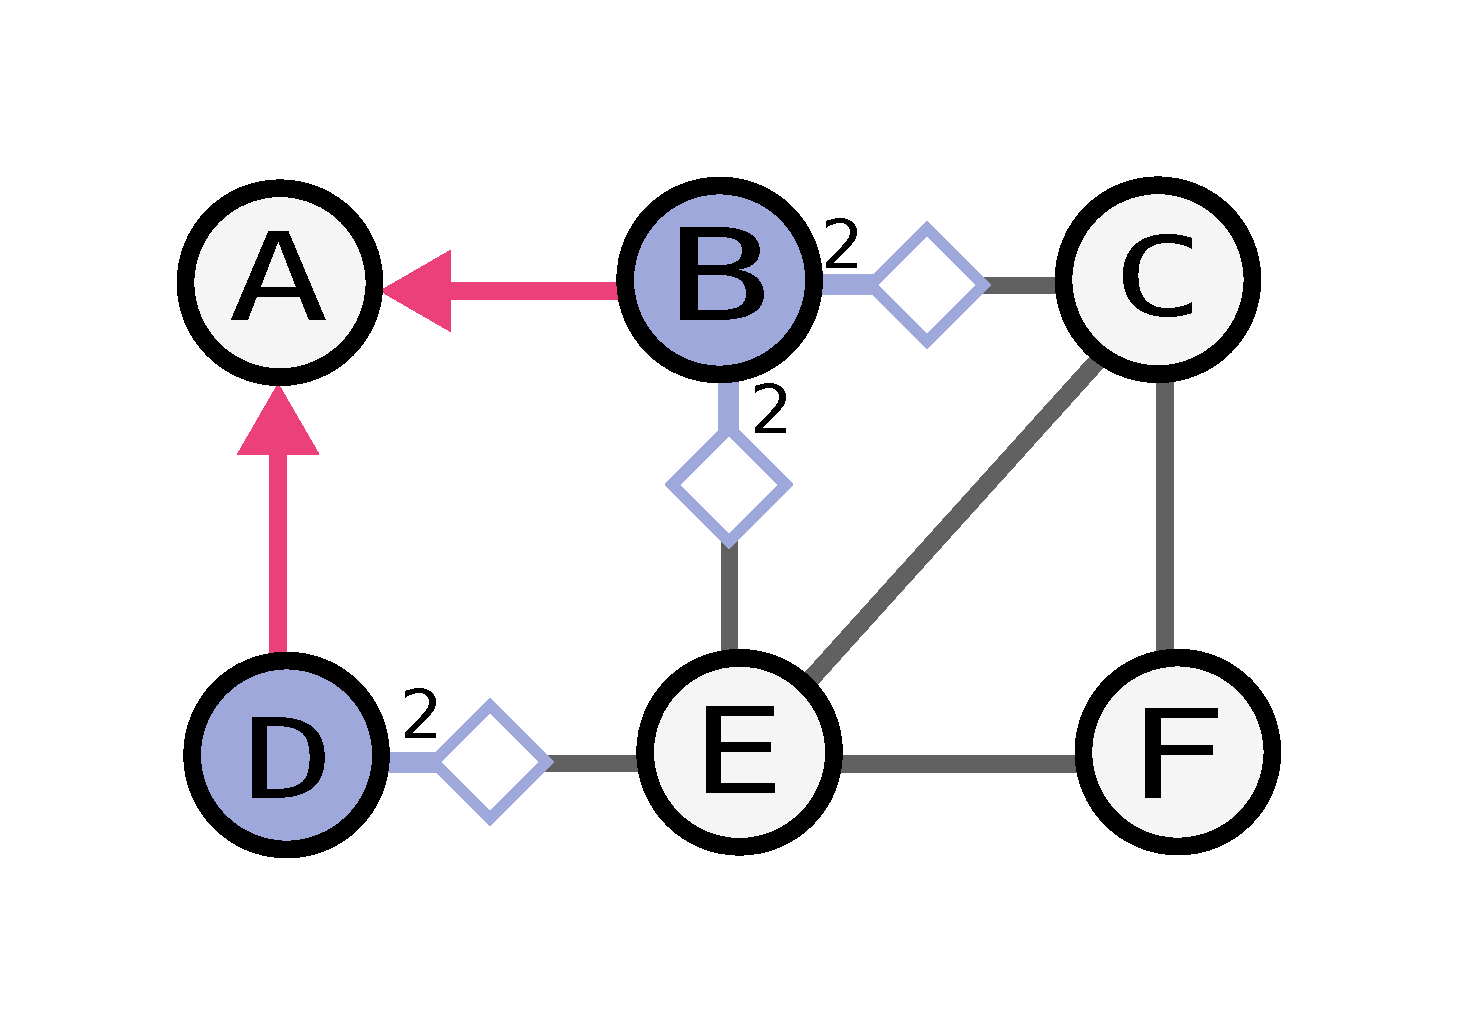
\includegraphics[width=0.5\paperwidth]{round2.pdf}
    \end{figure}
\end{frame}


\begin{frame}
    \frametitle{Example}
    \begin{figure}
    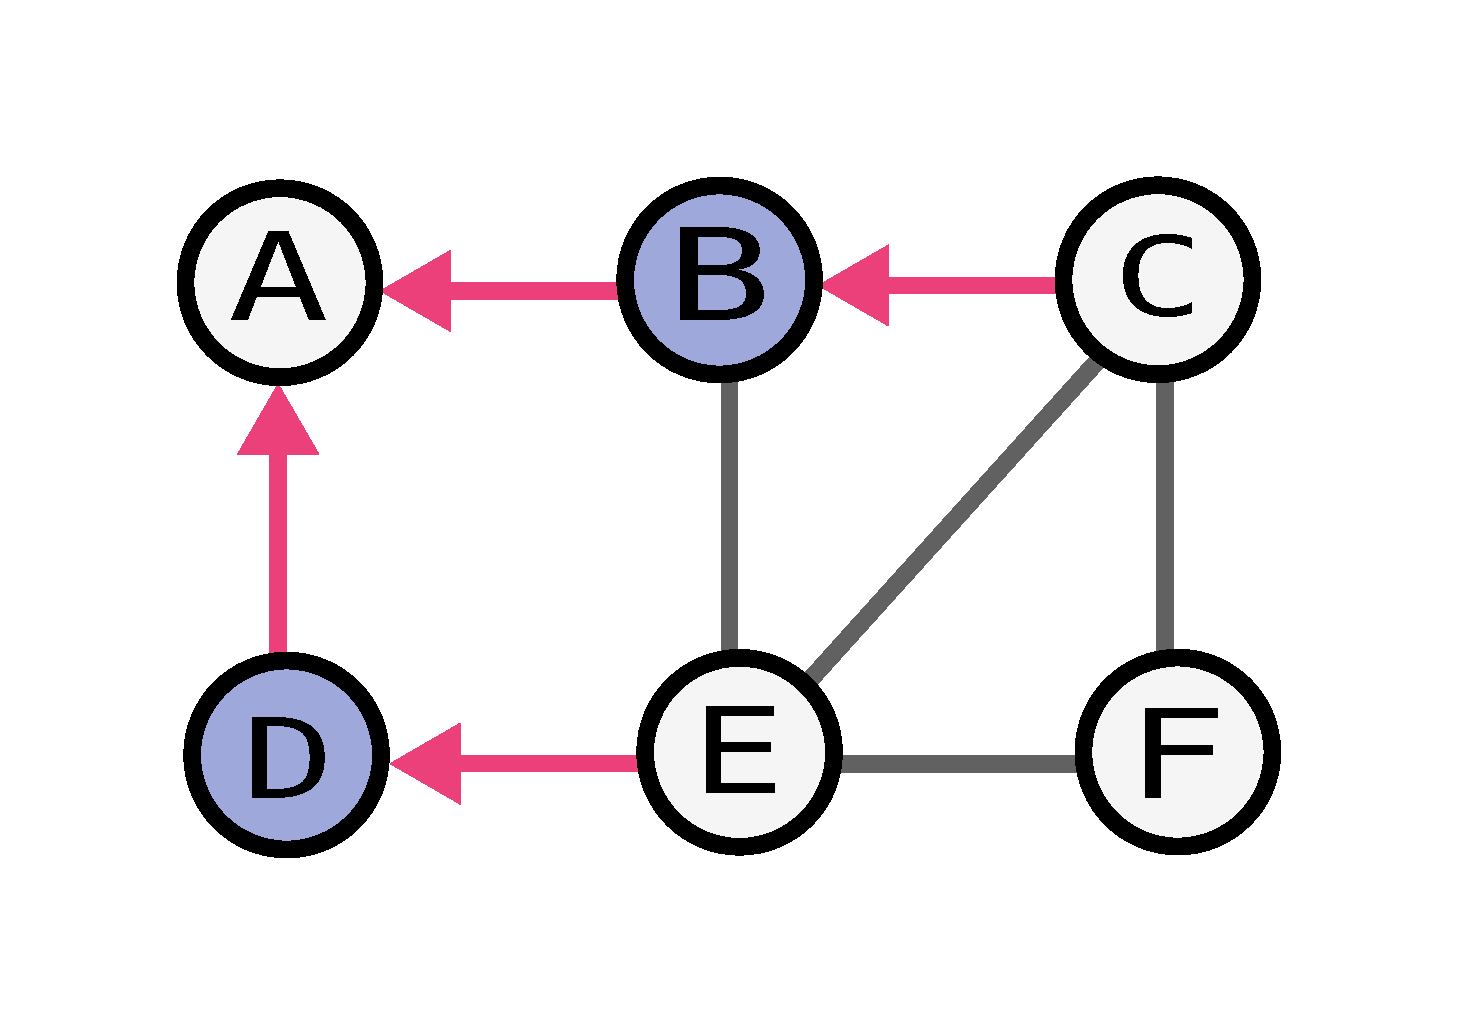
\includegraphics[width=0.5\paperwidth]{round2-end.pdf}
    \end{figure}
\end{frame}


\begin{frame}
    \frametitle{Example}
    \begin{figure}
    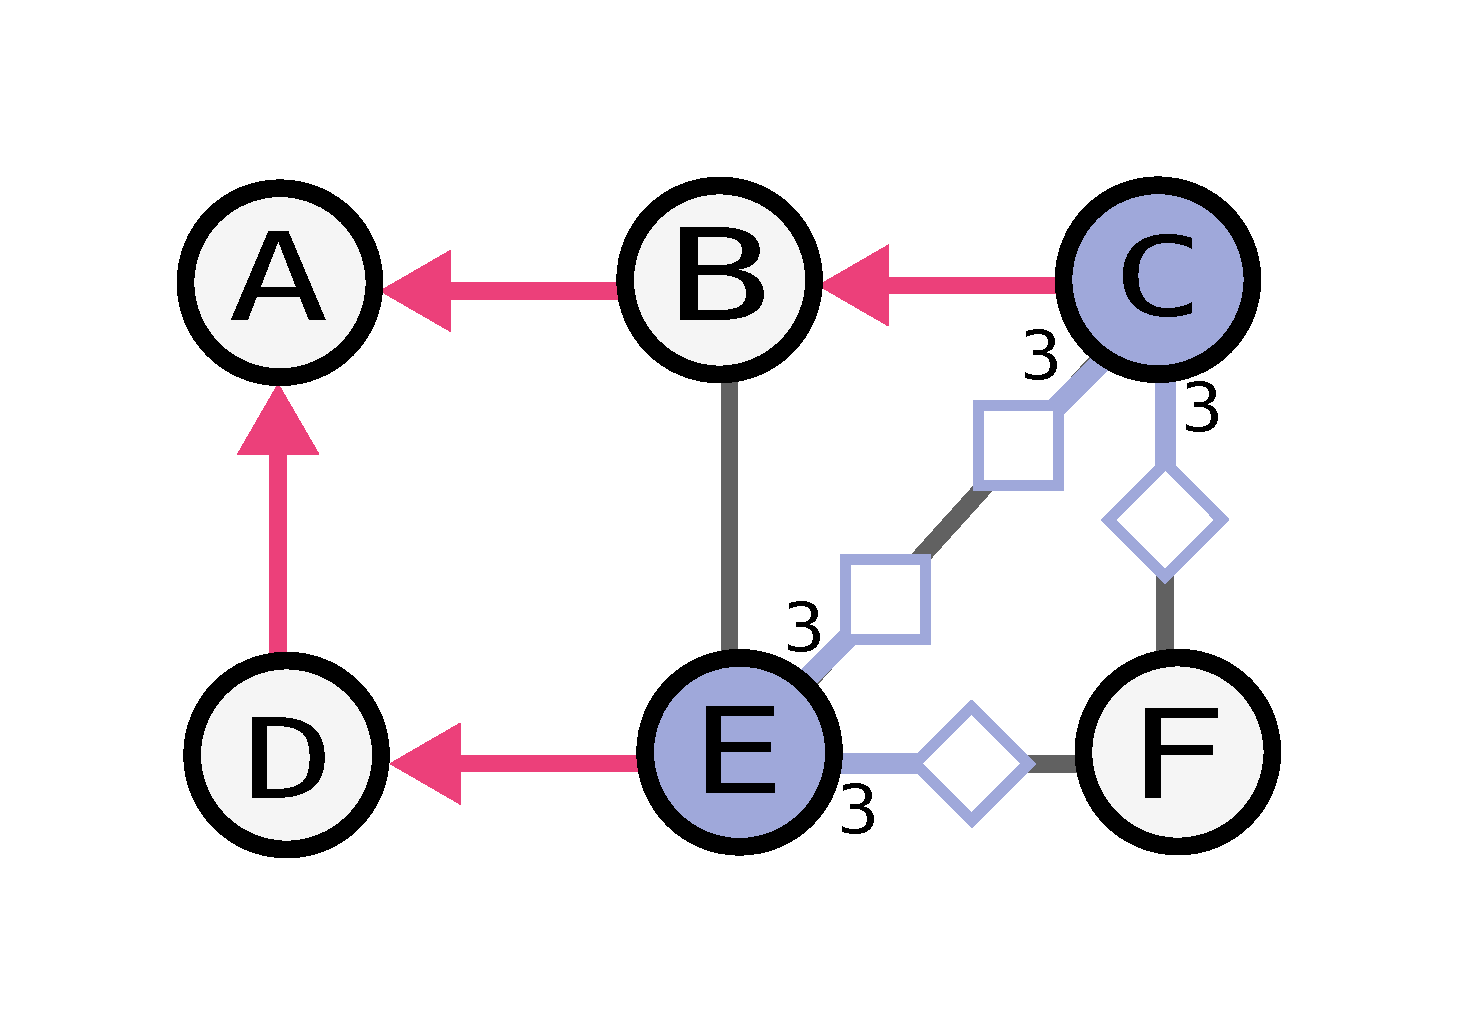
\includegraphics[width=0.5\paperwidth]{round3.pdf}
    \end{figure}
\end{frame}


\begin{frame}
    \frametitle{Example}
    \begin{figure}
    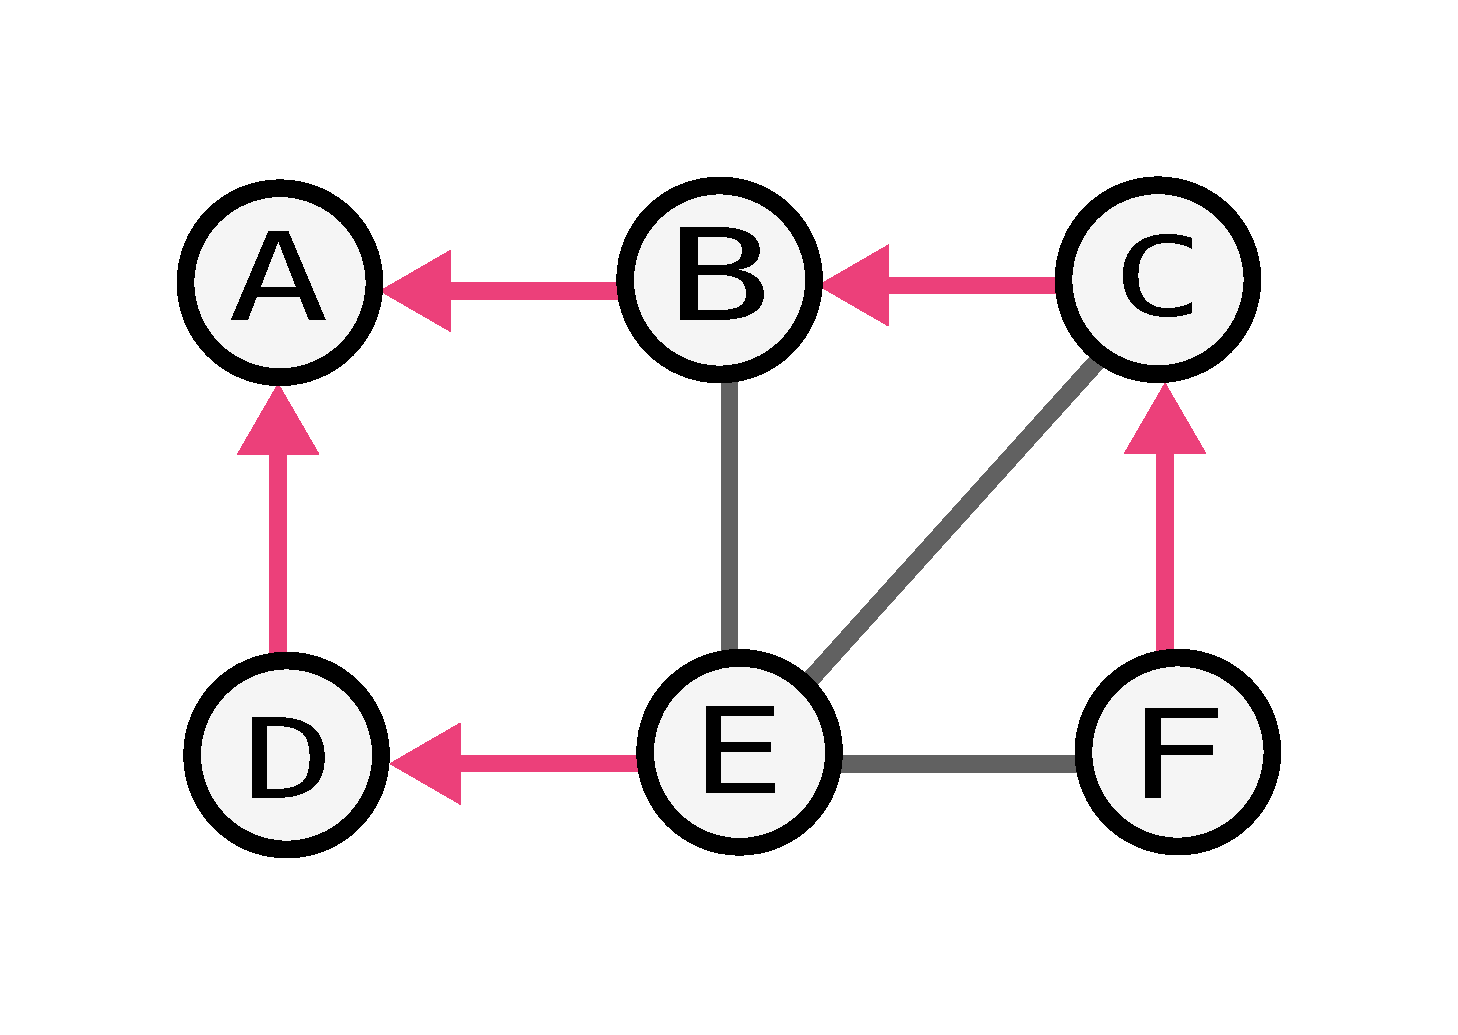
\includegraphics[width=0.5\paperwidth]{round3-end.pdf}
    \end{figure}
\end{frame}

\begin{frame}[fragile]
    \frametitle{Synchronous BFS (Pseudocode)}
    \begin{itemize}
        \item Assume root begins computation.
        \item Algorithm is synchronous.
    \end{itemize}
    \pause

    \begin{minted}{python}
    def bfs_spanning_tree(self):
    \end{minted}
    \pause
    \begin{minted}{python}
      if self.id == ROOT_ID:
        self.visited = True; self.depth = 0;
        for n in self.neighbours: n.send(self.id)
    \end{minted}
    \pause
    \begin{minted}{python}
      for round in range(1, DIAMETER+1):
        if not self.visited: # if visited, skip
    \end{minted}
    \pause
    \begin{minted}{python}
          if self.queries: # if we have a query
            # randomly choose from queries
            parent = random.choice(self.query)
            self.visited = True
            self.depth = round
    \end{minted}
    \pause
    \begin{minted}{python}
            # synchronous
            for n in self.neighbours: n.send(self.id)
        self.queries = [];
    \end{minted}
\end{frame}

\begin{frame}[fragile]
    \frametitle{Synchronous BFS (Ending earlier if visited)}

    \begin{minted}{text}
    def bfs_spanning_tree(self):
    \end{minted}
    \begin{minted}{text}
      if self.id == ROOT_ID:
        self.depth = 0;
        for n in self.neighbours: n.send(self.id)
    \end{minted}
    \begin{minted}{python}
        return # early-exit for root node
    \end{minted}
    \begin{minted}{text}
      for round in range(1, DIAMETER+1):
    \end{minted}
    \begin{minted}{text}
          if self.queries: # if we have a query
            # randomly choose from queries
            parent = random.choice(self.query)
            self.visited = True
            self.depth = round
    \end{minted}
    \begin{minted}{text}
            # synchronous
            for n in self.neighbours: n.send(self.id)
    \end{minted}
    \begin{minted}{python}
            return # early-exit for child
    \end{minted}
\end{frame}

\begin{frame}[fragile]
    \frametitle{Synchronous BFS (Learning children)}
    \begin{itemize}
        \item Assume root begins computation.
        \item Algorithm is synchronous.
    \end{itemize}

    \begin{minted}{text}
    def bfs_spanning_tree(self):
    \end{minted}
    \begin{minted}{text}
      if self.id == ROOT_ID:
        self.visited = True; self.depth = 0;
        for n in self.neighbours: n.send(self.id)
    \end{minted}
    \begin{minted}{text}
      for round in range(1, DIAMETER+1):
    \end{minted}
    \begin{minted}{python}
        if self.visited: # if visited, wait for children
          for q in self.queries: self.children.append(q)
    \end{minted}
    \begin{minted}{text}
        else: # if not visited, run code
          if self.queries: # if we have a query
            # randomly choose from queries
            parent = random.choice(self.query)
            self.visited = True
            self.depth = round
    \end{minted}
    \begin{minted}{text}
            # synchronous
            for n in self.neighbours: n.send(self.id)
    \end{minted}
    \begin{minted}{python}
            parent.send(self.id) # send to parent
    \end{minted}
    \begin{minted}{text}
        self.queries = [];
    \end{minted}
\end{frame}


\begin{frame}
    Thank you!
\end{frame}

\begin{frame}
    Thank you!
\end{frame}

\begin{frame}
    % Minimum weight spanning tree: synchronous (5.5.11, Kshemkalyani)
\end{frame}

\begin{frame}
    % Spanning tree computation: async version
\end{frame}


\begin{frame}
    % Converting bounded delay to synchronous (Gerard Tel, Chapter 12)
\end{frame}

\end{document}
